\subsection{GLSL}

\subsubsection{OpenGL}

OpenGL is a cross-platform API that has been an industry-standard ever since it was introduced in 1992\cite{glredbook}. Major decisions are made by the OpenGL Architecture Review Board, ARB. ARB was created by Silicon Graphics in 1992 and had representatives from SGI, Intel, Microsoft, Compaq, Digital Equipment Corporation, Evans \& Sutherland and IBM. Later on, companies such as 3Dlabs, Apple, ATI, Dell, IBM, Intel, nVIDIA and Sun Microsystems were added. OpenGL shares many characteristics of a previous API called Iris GL. It is designed in a way where it tries to be the lowest level interface for accessing graphics hardware but still provide hardware independence. OpenGL is supported in PC, Mac and Unix-systems.

\begin{figure}[ht!]
\centering
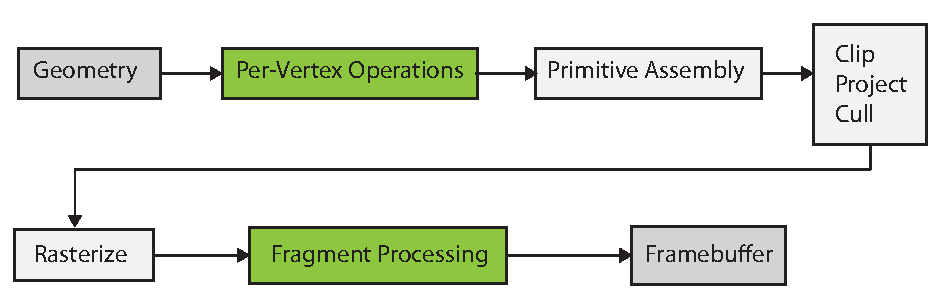
\includegraphics[width=100mm]{img/glpipeline.pdf}
\caption{OpenGL orginially had a fixed pipeline where non of these steps could be modified.}
\label{glfixed}
\end{figure}

Figure \ref{glfixed} shows the overview of the complete OpenGL pipeline in version 1.5 and earlier. It was said to have fixed functionality because every OpenGL implementation was required to have the same functionality. The set of operations and how they were applied were defined by the fixed OpenGL specification. The Fragment Processing step in Figure \ref{glfixed} is where each fragment gets its final value. A fragment can be thought of as the data needed to both shade the pixel decide if the fragment is to be displayed as a pixel (need information about depth, alpha). The fixed fragment stage could only handle tasks such as interpolating color values, texture mapping and fog. 

\subsubsection{The shading language}

In version 2.0, OpenGL introduced GLSL, the OpenGL shading language. With the OpenGL shading language, the fixed functionality stages for vertex and fragment processing (green steps in Figure \ref{glfixed}) could now be customized and programmed\cite{glshadinglanguage}. It was still possible to do everything that the previous fixed pipeline supported but it also gave the software developer the opportunity to alone control the output. The programs written in GLSL are called OpenGL shaders, vertex shaders or fragment shaders. The OpenGL Shading Language is a high-level procedural language based on C and C++ syntax and flow control. Vector and matrix types/operations is natively supported together with a set of  math functions commonly used in graphics shading.
\newline

\subsubsection{Shaders}

\begin{figure}[ht!]
\centering
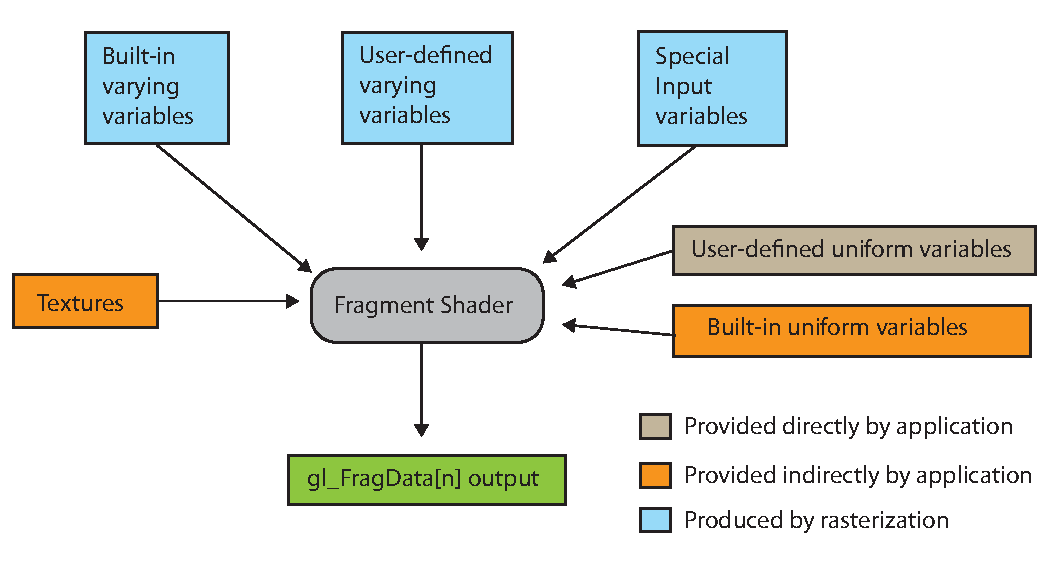
\includegraphics[width=100mm]{img/frag.pdf}
\caption{The inputs and outputs of a GLSL fragment shader.}
\label{glfrag}
\end{figure}

Shaders are compiled from an input source of text at runtime. They are later linked to an OpenGL program and become executable. In image processing, only the fragment shader is of importance. In a fragment shader, any image processing algorithm can be applied on an input image. A fragment shader operates on one fragment at a time. Fragment shaders must be written in such a way that they can operate simulationeusly. When a fragment shader is being executed, it has no knowledge about other fragments and their data. 
\newline

Figure \ref{glfrag} shows the inputs and outputs of a fragment processor. Some variables are built-in, specified by the OpenGL implementation. There is a notion of varying and uniform variables. Uniform variables are, as the name suggests, uniform across all shaders. Varying variables are defined per vertex in the vertex shader. Before processing each fragment, the hardware interpolates the geometry and gives the fragment shader the correct varying attributes. An example of a varying attribute is texture coordinates. The texture coordinates are defined at each vertex. Before the processing of the fragment shader, the texture coordinates are interpolated across the geometry and can be used later in the fragment shader to do texture lookups.

\renewcommand{\lstlistingname}{Code}
\begin{lstlisting}[caption= Example of adding two images in GLSL, label=glsl1]
uniform sampler2D texture0;
uniform sampler2D texture1;

uniform float scale;
varying vec2 texcoord;

void main()
{
    gl_FragData[0] = scale * (
        texture2D(texture0, texcoord) + 
        texture2D(texture1, texcoord));

}
\end{lstlisting}

Code \ref{glsl1} shows an example of fragment shader in GLSL that adds two images together. The images have been converted to OpenGL textures, \texttt{texture0} and \texttt{texture1}. The function \texttt{texture2D} together with the varying variable \texttt{texcoord} is used to fetch the data from a texture. The value is multiplied with the uniform value \texttt{scale} (same for all fragments) and finally written to the framebuffer through the built-in \texttt{gl\_FragData}. Syntax is similar to a C program and every fragment shader needs a \texttt{main} function.
